\documentclass[9pt,journal,a4]{IEEEtran}

\usepackage{cite}
\usepackage{amsmath}
\usepackage{graphicx}
\usepackage{textcomp}
\usepackage{booktabs}
\usepackage{stfloats}
\usepackage{balance}
\graphicspath{{figures/}}

\begin{document}

\title{Estimating Aggregated Heat-Pump Capacity from Net Load Using a Transferable Simultaneity Factor}

\author{Alexandre~M.~V.~Gouveia, Md. Umar Hashmi, Reinhilde D'hulst, Dirk Van Hertem}

\maketitle

\begin{abstract}
Distribution system operators (DSOs) meter the aggregated net load of a low-voltage feeder but rarely know how much electric thermostatic load (ETL), such as heat pumps, sits behind it. This paper estimates that population from net load and ambient temperature. Two temperature-response functions are fitted: an unsupervised bathtub curve on the metered net load, and a supervised simultaneity factor (SF) on submetered load. The net-load fit gives the coincident temperature-sensitive demand; the SF converts it into the summed non-coincident installed peak. The SF is empirically stable against a population's ETL rate and installed capacity, and its simultaneity sensitivity transfers across the two populations studied, so a curve calibrated on a submetered pilot serves that population's un-submetered feeders. From an observable net-load fit and a transferred SF, three quantities are derived: installed capacity, temperature-driven energy and a temperature-dependent power envelope bounding flexibility. Across Swiss substations resampled from one pool of smart meters, the installed capacity is recovered to a weighted absolute percentage error of 10\%; on a single German feeder held out of sample, the estimate reaches 17\%, falling to 7\% once the threshold temperature is read from the observable net-load fit. After calibration on a submetered pilot, applying the method to a target feeder requires only net load and ambient temperature, making the method suitable for aggregated ETL quantification in unobservable low voltage networks.
\end{abstract}

\begin{IEEEkeywords}
Electric thermostatic loads, heat pumps, low-voltage networks, simultaneity factor, installed capacity, smart meter data, distribution system observability.
\end{IEEEkeywords}


% =====================================================================
\section{Introduction}
\label{sec:intro}

The electrification of residential heating is a central lever of decarbonisation policy, and the heat pump (HP) is its main instrument. Its uptake is growing quickly, and with it the share of household demand that follows outdoor temperature rather than occupancy alone \cite{Vel11, Akm14}.

This uptake supports decarbonisation, yet it loads low-voltage (LV) networks that were not sized for it. Field and simulation studies show that HPs raise coincident feeder and transformer peaks, most sharply in cold weather, alongside electric vehicles and rooftop solar \cite{Akm14, Som21, Bec24, Lia26}. Planning and operating these networks depends on knowing how much thermostatic load sits behind each metering point.

A distribution system operator (DSO) rarely holds that information. It meters aggregated net load and can obtain weather, but seldom the consumer count, appliance registers or nameplate ratings needed to interpret the thermal response \cite{Gou26}. The installed capacity of the electric thermostatic loads (ETLs) behind a feeder is thus largely unobserved.

Four lines of research attempt to close this gap. Non-intrusive load monitoring and HP detection identify or disaggregate thermostatic load from customer meters \cite{Fei13, Wei20b, Ray19, Bru23, Gis26}, and have been extended to LV substations \cite{Wan20, Oma24}. These methods recover an energy time series or a present-absent label rather than the installed capacity, and the substation demonstrations remain largely synthetic.

Change-point and degree-day regression models load as a piecewise-linear function of temperature, from the canonical building-level formulations \cite{Fel08, Ruc92, Kis04, Faz16} to aggregated and smart-meter populations \cite{Ali11, Per17b, Mac19}. These recover heating and cooling sensitivities and a threshold temperature, but stop at the coincident response and do not reach the non-coincident installed sum.

Installed-capacity estimation of behind-the-meter assets is by contrast well developed for photovoltaics, where the capacity is inferred from aggregated net load or smart-meter data \cite{Tab18, Was21, Liu22, Azz23b, Gou25}, and even the service-transformer rating has been recovered this way \cite{Azz24}. The thermostatic-load counterpart is largely missing \cite{Gou26}.

The simultaneity of an aggregated HP population, and the coincident peak demand it produces, inform network planning, where they set the design load \cite{Lov17, Che21b, And20, Rou23} and bound the flexibility the population offers \cite{Mul19, Zir19}. These quantities are measured on submetered populations of known size and read as an input to planning, rather than recovered from an un-submetered feeder.

To the best of the authors' knowledge, no prior method estimates the installed capacity of an aggregated ETL population directly from feeder-level net load without submetering the target feeder. This paper addresses that gap. The contributions are threefold.
\begin{enumerate}
\item The fitted Simultaneity Factor (SF) of an aggregated ETL population is empirically stable against its ETL rate and installed capacity over the tested range. Across the two populations studied its simultaneity sensitivity transfers, while the threshold temperature follows local climate and is recovered from the observable net-load fit. This makes the SF, classically a submetered planning quantity, usable where no ETL is metered.
\item Building on this, the installed ETL capacity of an un-submetered feeder is estimated by combining an observable net-load fit with a transferred SF. Two further quantities, temperature-driven energy and a power envelope bounding flexibility, are derived from the same two fits; once the SF is calibrated on a submetered pilot, applying them to a target feeder needs only net load and temperature.
\item The fits and the capacity estimate are examined on a single real, physically aggregated feeder held out of sample. This case study separates what transfers across the two populations from what must be re-read locally, and reports the capacity error under a realistic, submetering-free application of the method.
\end{enumerate}

The rest of the paper is structured as follows. Section~\ref{sec:problem} states the problem; Section~\ref{sec:fits} presents the two fits; Section~\ref{sec:usecases} describes the use cases derived from them; Section~\ref{sec:results} reports numerical results on Swiss data; Section~\ref{sec:validation} validates on a real unseen feeder; Section~\ref{sec:discussion} discusses accuracy, generalisability and data requirements; Section~\ref{sec:conclusion} concludes.


% =====================================================================
\section{Problem Statement}
\label{sec:problem}

This paper addresses the quantification of ETLs at a metered point of an LV network, such as a substation or feeder. This metering point aggregates the load of consumers connected downstream of it, some of which might have ETL loads.

The net load is the sum of an ETL and a non-ETL component,
\begin{equation}
P_{\mathrm{net}}(t) = P_{\mathrm{ETL}}(t) + P_{\text{non-ETL}}(t),
\label{eq:decomp}
\end{equation}
where only the ETL component responds directly to temperature. The non-ETL component also has an indirect temperature response, as residential occupancy increases in severe cold or heat, adding load. However, the total temperature response is assumed to be dominated by ETLs and the non-ETL contribution is neglected. This assumption is further discussed in Section \ref{sec:discussion}.

The problem is to recover $P_{\mathrm{ETL}}(t)$ from the aggregated net load, and to estimate three quantities about the ETL population that aid DSO operation and planning: ETL installed capacity, their energy consumption and the bounds of their flexibility potential. Section~\ref{sec:fits} defines the functions which are fitted and used to quantify the aggregated ETL population, and Section~\ref{sec:usecases} derives the three quantities from them.


% =====================================================================
\section{Temperature-Response Functions}
\label{sec:fits}

Two functions are defined to describe the ETL population's behaviour with respect to ambient temperature. The first is fitted to the net load, which the DSO already meters, and recovers the response $P_{\mathrm{ETL}}(T)$ itself, without any label. The second is fitted to the SF of the aggregated ETLs, using submetered data. Both take the same piecewise-linear form, and both are fitted on daily means, which averages out the effects of building thermal inertia.


\subsection{Net-Load Function (Unsupervised)}
\label{sec:fits-net}

The aggregated net load of Equation~\eqref{eq:decomp} is fitted to temperature as
\begin{equation}
P_{\mathrm{net}}(T) = P_{\mathrm{base}} + s_h \max(0, T_h - T) + s_c \max(0, T - T_c),
\label{eq:bathtub}
\end{equation}
where $P_{\mathrm{base}}$ is the temperature-independent load [kW], $s_h$ and $s_c$ are the heating and cooling thermal sensitivities [kW/$^\circ$C], and $T_h \le T_c$ are the heating and cooling threshold temperatures [$^\circ$C] bounding a dead band over which no thermal response is present. The two arms are the ETL response $P_{\mathrm{ETL}}(T)$, and the flat term $P_{\mathrm{base}}$ is the non-ETL load of Equation~\eqref{eq:decomp}.

Equation~\eqref{eq:bathtub} is termed the bathtub function, after the shape of its two arms and flat centre. Where no electric cooling is present, $s_c$ is zero and the form reduces to a heating hockey stick, and where no electric heating is present only the cooling arm remains. This function is unsupervised, since it needs only the net load and the ambient temperature the DSO already holds, and no submetered or labelled ground truth. Fig.~\ref{fig:bathtub} shows the full bathtub form recovered from aggregated smart meter data from Austin, Texas \cite{pecanstreet}, with the parameters of Equation~\eqref{eq:bathtub} marked on the curve.

\begin{figure}[t]
\centering
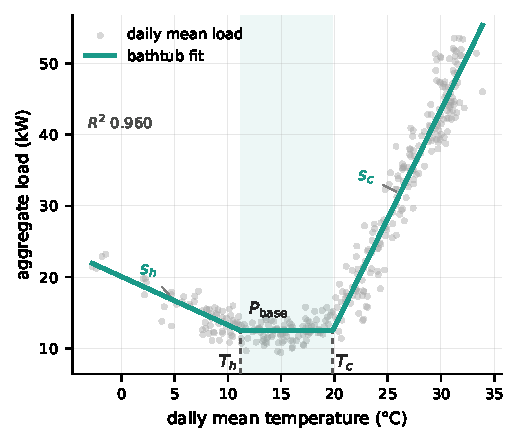
\includegraphics[width=\columnwidth]{figures/fig_bathtub_example.pdf}
\caption{Equation~\eqref{eq:bathtub} fitted to an aggregate of air-conditioned and furnace-heated dwellings in Austin, Texas \cite{pecanstreet}. The parameters are marked on the curve: the base load $P_{\mathrm{base}}$, the heating and cooling threshold temperatures $T_h$ and $T_c$ bounding the dead band (shaded), and the heating and cooling slopes $s_h$ and $s_c$.}
\label{fig:bathtub}
\end{figure}


\subsection{Simultaneity-Factor Function (Supervised)}
\label{sec:fits-sf}

The second function characterises the synchronous behaviour, or simultaneity, of the ETL population. The SF is the fraction of the population's installed capacity drawn at a given time $t$,
\begin{equation}
\mathrm{SF}(t) = \frac{P_{\mathrm{ETL}}(t)}{P_{\mathrm{ETL}}^{\max}},
\label{eq:sf}
\end{equation}
where $P_{\mathrm{ETL}}^{\max}$ is the installed capacity, operationalised as the sum of the individual ETLs' peak electrical demand, taken here as the 99.9th percentile of each submetered series. This is an empirical maximum draw rather than a nameplate rating; the two differ for variable-speed units, and the peak-demand definition is the quantity that sizes a feeder. The SF is bounded in $[0,1]$ and, unlike the net load, is built from the submetered ETL load, which is usually not known to the DSO. This function is therefore supervised, calibrated on submetered ground truth.

The SF is fitted to temperature in the same hockey-stick form as the heating arm of Equation~\eqref{eq:bathtub},
\begin{equation}
\mathrm{SF}(T) = b + m \max(0, T_h^{\mathrm{SF}} - T),
\label{eq:sffit}
\end{equation}
with $b$ a small base fraction, $m$ the simultaneity sensitivity [1/$^\circ$C] and $T_h^{\mathrm{SF}}$ the threshold temperature of the SF, analogous to $T_h$ of Equation~\eqref{eq:bathtub} but fitted separately. Fig.~\ref{fig:sf} shows the function for an HP population on Swiss data \cite{Bru25,Kai26b}.

\begin{figure}[t]
\centering
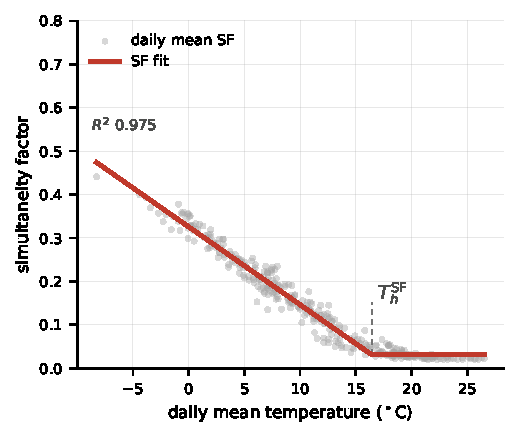
\includegraphics[width=\columnwidth]{figures/fig_sf_example.pdf}
\caption{Equation~\eqref{eq:sffit} fitted to the SF of an HP population on Swiss data \cite{Bru25,Kai26b}, with the threshold temperature $T_h^{\mathrm{SF}}$ marked. The factor is bounded in $[0,1]$ and rises as temperature falls.}
\label{fig:sf}
\end{figure}

The two functions are complementary. The net-load function is observable but mixes the ETL and non-ETL loads in its slope, whereas the SF function is not observable without submetering but isolates the ETL simultaneity. Section~\ref{sec:usecases} combines them, the net-load function supplying the coincident ETL peak and the SF function scaling it to installed capacity and flexibility.


% =====================================================================
\section{Use Cases of the Functions}
\label{sec:usecases}

The two functions described in Section~\ref{sec:fits} can be used to extract three quantities a DSO needs about the ETL population: its total installed capacity, its energy consumption and its flexibility potential. Energy consumption is derived from the net-load function only. Installed capacity and flexibility additionally require the SF function, since the net load exposes a coincident demand rather than the non-coincident sum of the individual peak demands. Each use case is a relation between the fitted parameters, stated here and evaluated in Section~\ref{sec:results}.


\subsection{ETL Installed Capacity Estimation}
\label{sec:uc-capacity}

The installed capacity $P_{\mathrm{ETL}}^{\max}$ is the sum of the individual peak demands of Section~\ref{sec:fits-sf}, which the aggregated ETLs never draw at once, so the net load never exposes it directly. What the net-load function does expose is the coincident demand $P_{\mathrm{ETL}}(T)$ at any temperature. Evaluated at the coldest recorded temperature, $T_{\min}$, it gives the coincident peak $P_{\mathrm{ETL}}(T_{\min})$.

Rearranging the SF definition of Equation~\eqref{eq:sf}, the installed capacity follows from that peak and the SF at the same temperature,
\begin{equation}
P_{\mathrm{ETL}}^{\max} = \frac{P_{\mathrm{ETL}}(T_{\min})}{\mathrm{SF}(T_{\min})}.
\label{eq:capacity}
\end{equation}
The net-load function supplies the numerator, which the DSO observes, and the SF function supplies the denominator, which is transferred from a submetered reference population where it is not available locally. The estimate is therefore only as good as the transferred simultaneity, a dependence that is tested in Sections~\ref{sec:results} and \ref{sec:validation}.


\subsection{ETL Energy Consumption Estimation}
\label{sec:uc-energy}

The energy the ETL population draws over a period follows from integrating its temperature response over that period. The heating arm of the net-load function gives the ETL power $P_{\mathrm{ETL}}(T) = s_h \max(0, T_h - T)$, and over a day of mean temperature $T$ the temperature-driven ETL energy is that power across the hours it applies,
\begin{equation}
E_{\mathrm{ETL}} = s_h \max(0, T_h - T)\,\Delta t,
\label{eq:energy}
\end{equation}
with $\Delta t$ the length of the period. Only the net-load function is needed. Given a measured temperature, the arm disaggregates the ETL power $P_{\mathrm{ETL}}(t)$ from the net load $P_{\mathrm{net}}(t)$; given a forecast temperature, it forecasts that power for a future period.

The dead band bounds the estimate. Above $T_h$ the arm is zero, so any ETL energy that persists into mild weather, most plausibly domestic hot water, is unrepresented by construction. The energy reported is consequently the temperature-driven share rather than the annual total.


\subsection{Flexibility Potential}
\label{sec:uc-flex}

The flexibility an HP population offers is bounded by the gap between what it can draw and what it draws. At temperature $T$ the population draws the coincident demand $P_{\mathrm{ETL}}(T) = \mathrm{SF}(T)\,P_{\mathrm{ETL}}^{\max}$ and leaves the remainder of its installed capacity idle,
\begin{equation}
P_{\mathrm{flex}}(T) = \big(1 - \mathrm{SF}(T)\big)\,P_{\mathrm{ETL}}^{\max}.
\label{eq:flex}
\end{equation}
This is the upward headroom available to a DSO for demand response, while the drawn part $P_{\mathrm{ETL}}(T)$ is the load available to shed. This use case uses both functions: the SF function gives the idle and drawn fractions against temperature, and the capacity of Equation~\eqref{eq:capacity} scales them to kilowatts.

The bound is an envelope rather than a dispatchable quantity, since it ignores the thermal state of each dwelling and the comfort limits within which its HP can be shifted. It is reported as a potential against temperature, not as a firm reserve.


% =====================================================================
\section{Numerical Results}
\label{sec:results}


\subsection{Dataset and Substation Design}
\label{sec:data}

The data used in this section is a combination of two Swiss sources, the HEAPO dataset \cite{Bru25} and an additional smart-meter dataset \cite{Kai26b}, pooled into one set of LV consumers. The ETL used throughout is the HP. Other ETLs are present in the dataset, but these are only flagged, not submetered, and are thus withheld. The load profiles have 15-minute resolution, while ambient temperature is hourly, which sets one hour as the finest resolution at which the functions are fitted.

Synthetic substations are drawn from this pool by iterating over a size and ETL rate grid. The number of consumers $N$ and the number of HPs $N_{hp}$ are each capped at 50, and every feasible cell of the grid, with $N_{hp} \leq N$, is filled with the same number of replicates, giving 1000 substations. The HPs and the base households are drawn as two independent samples with replacement, which decouples the HP count from the household composition. Each substation is tied to a single station, so one temperature series applies to all of its members.

Two error metrics recur below. The weighted absolute percentage error (WAPE) scores an estimate $\hat{y}_i$ against its ground truth $y_i$ across the substations $i$,
\begin{equation}
\mathrm{WAPE} = \frac{\sum_i |\hat{y}_i - y_i|}{\sum_i y_i} \times 100\%,
\label{eq:wape}
\end{equation}
so each substation is weighted by its true magnitude rather than equally. A small aggregate, whose percentage error is large but whose absolute error is small, therefore cannot dominate, and the metric reports the total error across a set of feeders as a DSO would read it. The median ratio, the median of $\hat{y}_i / y_i$, gives the direction of the error, below one for an underestimate and above one for an overestimate.

\subsection{Function Fits}
\label{sec:res-ff}

Both functions are fitted to each substation's aggregate, and their quality, measured by the $R^2$ that gives the share of variance the fit explains, climbs with aggregation in time and in space.

Averaging the load over longer windows removes the occupancy swings and building thermal inertia that do not track temperature. The net-load fit rises from a median $R^2$ of 0.74 at hourly resolution to 0.95 at daily, and the SF fit from 0.81 to 0.97, climbing monotonically through the four-, eight- and sixteen-hour windows in between. The daily mean, used throughout, sits at the top of this curve.

Spatial aggregation acts the same way, as more meters average out the load that is not thermal. At daily resolution the net-load fit rises from a median $R^2$ of 0.92 behind ten consumers to 0.96 behind fifty, and more steeply with the HPs whose signal it recovers, from 0.88 at five HPs to 0.97 at fifty. The SF fit, built from the HPs alone, rises with their number from 0.95 to 0.97 (the $R^2$ column of Table~\ref{tab:sf}, grouped by $N_{hp}$).


\subsection{Simultaneity Factor: Invariance and Transfer}
\label{sec:res-sf}

Beyond fitting well, the SF fit is stable. Its coldest-day SF and sensitivity $m$, reported in Table~\ref{tab:sf} as a median with its interquartile spread per $N_{hp}$ group, show no meaningful association with the substation's ETL rate or installed capacity over the tested range: $m$ holds near $0.016~^\circ$C$^{-1}$ and the maximum SF, on the coldest day, near 0.42 (Spearman $|\rho| < 0.08$ against either). More HPs behind the meter do not shift these values but tighten them, as the interquartile spread narrows with $N_{hp}$. The SF is thus a population coincidence, describing how HPs behave against temperature rather than how many or how dense they are.

This stability lets a curve calibrated on submetered substations serve un-submetered ones from the same population, and two splits bracket what the transfer buys. A substation-level split, in which the calibration and evaluation substations are resampled from one pool and therefore share households, reproduces the held-out SF at a median $R^2$ of 0.945 and recovers the coldest-day coincidence to a peak-SF WAPE that falls from 16\% at five HPs to 4\% at fifty (Table~\ref{tab:sf}); this measures reproducibility within the pool rather than independent generalisation. A stricter household-disjoint split, which partitions the 50 HPs of the largest station into two halves so that no HP informs both curves, gives a median $R^2$ of 0.93 [0.92, 0.95] and a peak-SF WAPE of 12\% [9, 15] over 120 random splits. The three-point gap in WAPE between the two is the price of genuine household independence.

A submetered pilot therefore carries a population's ETL simultaneity onto its un-submetered feeders to within roughly ten to twelve percent, and to a few percent once tens of HPs aggregate, which Section~\ref{sec:res-capacity} uses to estimate installed capacity.

\begin{table}[t]
\centering
\caption{Per-substation fitted SF parameters and transfer error by number of aggregated HPs $N_{hp}$}
\label{tab:sf}
\begin{tabular}{rcccc}
\toprule
$N_{hp}$ & $R^2$ & SF$_{\mathrm{cold}}$ & $m$ ($^\circ$C$^{-1}$) & peak-SF WAPE (\%) \\
\midrule
5 & 0.954 & 0.42\,(0.12) & 0.016\,(0.005) & 16.4 \\
10 & 0.963 & 0.43\,(0.07) & 0.017\,(0.003) & 10.3 \\
20 & 0.970 & 0.43\,(0.06) & 0.016\,(0.002) & 8.2 \\
30 & 0.972 & 0.42\,(0.04) & 0.016\,(0.002) & 6.7 \\
40 & 0.973 & 0.42\,(0.04) & 0.016\,(0.002) & 5.4 \\
50 & 0.973 & 0.43\,(0.04) & 0.016\,(0.002) & 4.3 \\
\midrule
all & 0.968 & 0.42\,(0.06) & 0.016\,(0.003) & 10.2 \\
\bottomrule
\end{tabular}
\end{table}


\subsection{Installed Capacity Estimation}
\label{sec:res-capacity}

Equation~\eqref{eq:capacity} estimates the installed capacity from two fitted quantities. The numerator is the coincident peak $P_{\mathrm{ETL}}(T_{\min})$, read from the substation's own net-load fit at its coldest day, which the DSO observes. The denominator is the coldest-day SF, transferred as the reference median of Section~\ref{sec:res-sf} rather than measured. The target substation is therefore never submetered.

Table~\ref{tab:capacity} scores three estimators on the held-out half by the WAPE, the median ratio and the fit quality $R^2$. The transferred-SF estimator of Equation~\eqref{eq:capacity} recovers the installed capacity at a WAPE of 10\% and an $R^2$ of 0.97, with a slight 6\% overestimate at a median ratio of 1.06. A through-origin regression of capacity on the same net-load peak, fitted on the reference half, does no better at a WAPE of 10\% and matches the labels the transferred-SF route never uses. Its slope, 2.33, sits within two percent of the transferred $1/\mathrm{SF}$ of 2.36, so the physical estimator and the label-based regression are the same line.

Dividing instead by each substation's own coldest-day SF, an oracle a DSO could reach only with local submetering, sharpens the estimate to a WAPE of 6\% at an $R^2$ of 0.99 (Table~\ref{tab:capacity}). The four-point gap is the price of transferring the coincidence rather than measuring it, and the remainder is the net-load numerator. The error shrinks with aggregation, the transferred-SF WAPE falling from 29\% at five HPs to 5\% at fifty, as the noisy fits of a small draw settle. Part of the overestimate is the non-ETL temperature response the net-load fit adds to the heating arm, the neglected term of Equation~\eqref{eq:decomp} discussed in Section~\ref{sec:discussion}.

\begin{table}[t]
\centering
\caption{Installed-capacity accuracy on the held-out substations for three estimators}
\label{tab:capacity}
\begin{tabular}{lccc}
\toprule
estimator & WAPE (\%) & median ratio & $R^2$ \\
\midrule
Eq.~\eqref{eq:capacity}, transferred SF & 10.3 & 1.06 & 0.969 \\
regression benchmark & 10.1 & 1.04 & 0.970 \\
oracle (own SF) & 6.2 & 1.03 & 0.986 \\
\bottomrule
\end{tabular}
\end{table}


\subsection{Energy Consumption Estimation}
\label{sec:res-energy}

Equation~\eqref{eq:energy} needs only the net-load-fitted function. The heating arm, integrated over the year, gives the temperature-driven HP energy, which is tested here against the substation's own submetered HP load. Across the 1000 substations the estimate tracks the submetered energy with a Pearson correlation of 0.99, but underestimates it by a median 12\% (a median ratio of 0.88) at a WAPE of 15\%.

The energy estimator has two resolutions: one for the net-load fit and one for the temperature integration. Table~\ref{tab:energy} reports the WAPE and the median estimated-to-actual energy ratio, which falls below one when the estimate runs low, for each combination. Integrating the daily-fitted arm over the hourly temperature series, rather than the daily mean, lifts the ratio from 0.88 to 0.92 and the WAPE from 15\% to 12\%. A day whose temperature crosses the threshold holds more heating-degree-hours than its single-point mean implies. Refitting the arm at hourly resolution instead degrades the estimate, to a ratio of 0.86, since the sub-daily load is noisier than its daily mean (Section~\ref{sec:res-ff}). The daily fit integrated over the finer temperature series is therefore the best combination.

\begin{table}[t]
\centering
\caption{Energy-estimate accuracy against submetered HP energy, by the resolution of the fit and of the temperature integration}
\label{tab:energy}
\begin{tabular}{lcc}
\toprule
fit + integration & WAPE (\%) & median ratio \\
\midrule
daily + daily & 15.3 & 0.88 \\
hourly + hourly & 15.4 & 0.86 \\
daily + hourly & 12.4 & 0.92 \\
\bottomrule
\end{tabular}
\end{table}

The estimate is temperature-driven by construction, so the dead band bounds it. About 7\% of the HP energy is drawn above the threshold temperature, in mild weather where the heating arm is zero and most plausibly domestic hot water. Measured against this temperature-driven share alone, on the days below the threshold temperature, the estimate tightens to a WAPE of 10\% at a ratio of 0.94. Equation~\eqref{eq:energy} therefore estimates the temperature-driven energy rather than the annual total, the dead-band limit anticipated in Section~\ref{sec:uc-energy}.

Aggregation acts on the spread of the error, not its centre. Fig.~\ref{fig:energy-error} shows the signed error across substations, right-skewed with a median of $-12\%$, and its evolution with the HP count. The interquartile spread falls from 31\% at five HPs to 3\% at fifty, as the load that is not thermal averages out. The median underestimate does not follow it down but deepens to about $-16\%$, arguably as the non-ETL response that offsets it at a low ETL rate fades. More HPs therefore sharpen the estimate around a biased centre rather than removing the bias.

\begin{figure*}[t]
\centering
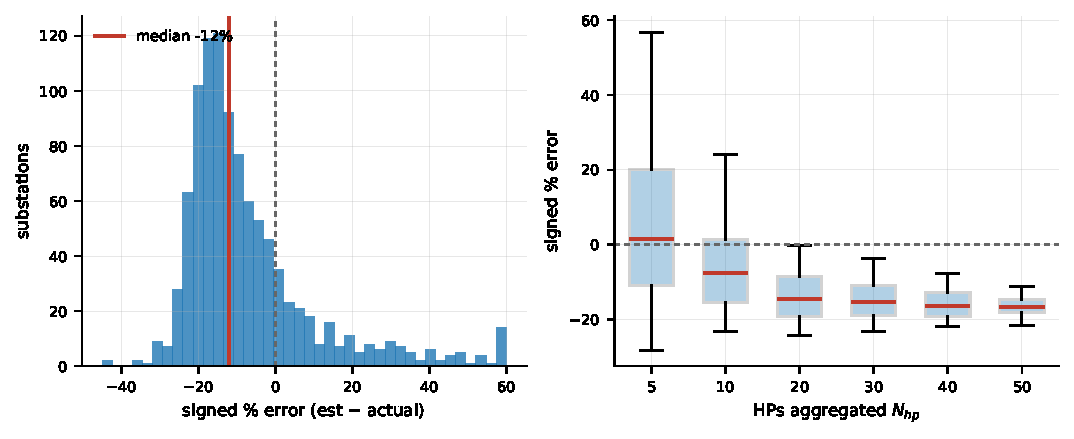
\includegraphics[width=\textwidth]{figures/fig_energy_error.pdf}
\caption{Signed percentage error of the energy estimate across the 1000 substations (left), and its distribution by number of aggregated HPs (right). Boxes show the interquartile range, whiskers the 5th--95th percentiles and the line the median.}
\label{fig:energy-error}
\end{figure*}


\subsection{Flexibility Potential}
\label{sec:res-flex}

Equation~\eqref{eq:flex} combines both functions: the transferred SF gives the fraction of installed capacity the population draws at each temperature, and the capacity of Equation~\eqref{eq:capacity} scales the idle remainder to kilowatts.

The SF, stable across the design, fixes the shape of the envelope. At the coldest day the population draws a median 42\% of its installed capacity, the coldest-day SF of Table~\ref{tab:sf}, so 58\% stands idle as upward headroom for demand response. The drawn fraction falls with temperature, to about 29\% at 0\,$^\circ$C and to about 3\% in mild weather, the base term $b$, where almost the whole capacity sits idle. The envelope is thus two-sided for a DSO. The load available to shed peaks in the cold, when the network is most stressed, at some 42\% of installed capacity, while the idle headroom grows largest in mild weather, when it is least useful.

As a fraction of installed capacity the envelope rests on the stable SF alone; scaled to kilowatts it inherits the capacity estimate's error of Section~\ref{sec:res-capacity}. It also ignores the thermal state of each dwelling and the comfort limits within which an HP can be shifted, so it is an illustrative upper bound on flexibility rather than a dispatchable quantity.


% =====================================================================
\section{Validation on a Real Unseen Feeder}
\label{sec:validation}

The Swiss results rest on synthetic aggregates of one population. A stronger test applies the method to a real feeder from another country, physically aggregated at its metering point and never seen in any fit. The feeder used here for that purpose is a German LV feeder from the WPUQ measurement campaign \cite{Sch22}, with 37 metered (and submetered) consumers and a measured installed HP capacity of 239~kW. The net-load fit (Section~\ref{sec:fits-net}) uses the feeder's own metered load, and the SF fit (Section~\ref{sec:fits-sf}) is transferred from the Swiss reference curve of Section~\ref{sec:res-sf}. Submetered data is only used for validation of results, and is not used as input in this section.

Both fitted functions carry to the real feeder (Fig.~\ref{fig:real-feeder}). The net-load hockey stick fits at an $R^2$ of 0.84 and the SF hockey stick at 0.83, close to the Swiss medians despite the change of country and the single physical aggregate. The forms are therefore not an artefact of the synthetic design.

The transfer splits into a part that carries and a part that does not. The simultaneity sensitivity is almost identical across the two countries, at $0.0162~^\circ$C$^{-1}$ on the feeder against $0.0161$ for Switzerland, so the slope of the SF transfers. However, the feeder's SF saturates at $13~^\circ$C against the Swiss $16~^\circ$C, a milder-climate shift of about three degrees. At the feeder's coldest day, near $-5~^\circ$C, the transferred Swiss curve therefore reads an SF of 0.38 where the true value is 0.32.

The net-load fit gives a coincident peak of 75~kW; scaled by the transferred Swiss SF of 0.38 it yields an installed capacity of 199~kW, an underestimate of 17\% against the measured 239~kW. The threshold temperature, though, need not be borrowed. The net-load fit already places it, at $13.9~^\circ$C on this feeder, and across the Swiss substations the net-load and SF threshold temperatures coincide to a median of $0.1~^\circ$C. Transferring only the SF slope and reading the threshold temperature from the observable net-load fit lifts the estimate to 222~kW, within 7\%, and needs no submetering anywhere. The oracle that divides by the feeder's own SF reaches 233~kW, within 2\%, which confirms the net-load numerator and the capacity relation are sound.

A sensitivity test removes HP circuits from the feeder, one subset at a time, leaving the 37 households and their base load in place. Table~\ref{tab:feeder-sweep} sweeps the retained count $N_{hp}$ and reports the signed median capacity error under the transferred and hybrid curves and the energy error, each over 200 random subsets. The hybrid capacity error is the smallest, within about 7\% for ten HPs and above. The energy error changes sign, from a 48\% overestimate at five HPs to the 15\% underestimate at full count. This shift is due to the non-ETL response inflating the estimate at low HP count, while neglecting consumption in the temperature dead-band dominates at higher HP count. The coldest-day SF holds near 0.32 whatever the count, so the power envelope keeps its shape while its kilowatts scale with the smaller capacity. Estimates from a handful of HPs are the least reliable, swinging with which circuits remain, so the method is best trusted on feeders that aggregate tens of them.

\begin{table}[t]
\centering
\caption{Use-case estimates on the real feeder as HP circuits are removed, at a fixed 37-house base. Signed median error over 200 random subsets per count}
\label{tab:feeder-sweep}
\begin{tabular}{rccc}
\toprule
$N_{hp}$ & capacity, transf.\ (\%) & capacity, hybrid (\%) & energy (\%) \\
\midrule
5 & +10 & +9 & +48 \\
10 & -5 & -0 & +9 \\
15 & -11 & -4 & -2 \\
20 & -14 & -6 & -8 \\
25 & -15 & -6 & -11 \\
30 & -16 & -7 & -14 \\
37 & -17 & -7 & -15 \\
\bottomrule
\end{tabular}
\end{table}

\begin{figure*}[t]
\centering
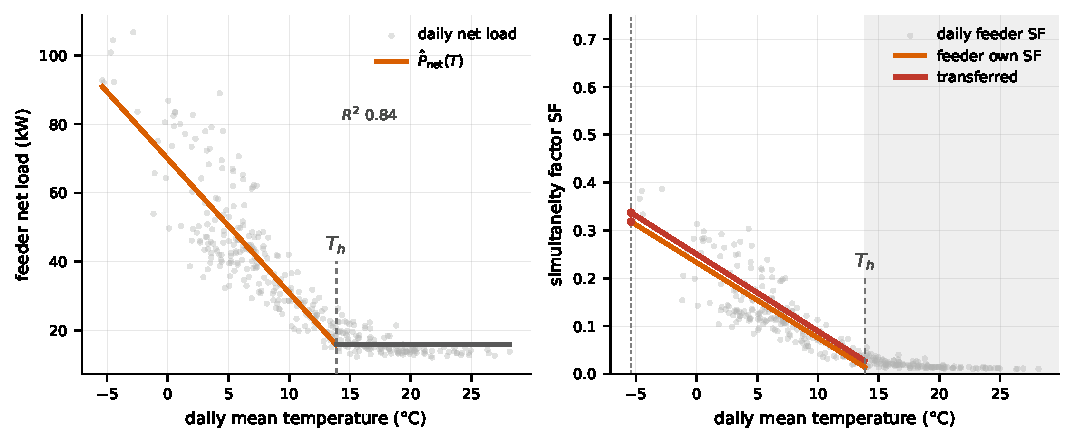
\includegraphics[width=\textwidth]{figures/fig_real_feeder.pdf}
\caption{The two functions fitted to the real German feeder. Left: the net-load hockey stick. Right: the feeder's own SF fit against the Swiss curve transferred to it and the hybrid curve that keeps the Swiss slope but takes its threshold temperature from the observable net-load fit; the sensitivity matches while the threshold temperature sits about three degrees lower, and the markers give the coincidence at the feeder's coldest day under each curve.}
\label{fig:real-feeder}
\end{figure*}


% =====================================================================
\section{Discussion}
\label{sec:discussion}

\subsection{Accuracy}

The capacity estimate carries two error sources, both traced in the results. The net-load numerator is biased by the non-ETL temperature response that Equation~\eqref{eq:decomp} neglects. At a low ETL rate this occupancy-driven load inflates the heating slope, and the energy estimate turns from a 12\% underestimate at a full ETL rate to an overestimate as the HPs thin out (Table~\ref{tab:feeder-sweep}). A zero-HP control makes this concrete: aggregating only HP-free households, the net-load fit still shows a small heating slope, and Equation~\eqref{eq:capacity} infers about 0.37~kW of spurious capacity per household where no HP exists. This floor is small per home but grows with feeder size, so it dominates the estimate at a low ETL rate and is negligible once HPs supply most of the temperature-driven load. The SF denominator carries the transfer error, which the real feeder shows to be the threshold temperature rather than the slope. On the synthetic held-out set the capacity WAPE is 10\%; on the real feeder the deployable estimate reaches 17\%, falling to 7\% once the threshold temperature is read from the observable net-load fit. A through-origin regression on the net-load peak does no better than Equation~\eqref{eq:capacity}, and its fitted coefficient recovers $1/\mathrm{SF}$, so the physical estimator matches it while needing no capacity labels.

\subsection{Generalisation}

The SF generalises in a specific and testable way. Within a population it is empirically stable against ETL rate and installed capacity over the tested range, so a curve from a submetered pilot serves that population's un-submetered feeders. Across populations the sensitivity $m$ transfers, at $0.0161$ against $0.0162~^\circ$C$^{-1}$ between the Swiss and German data, while the threshold temperature follows the local climate and must be set locally. The net-load fit supplies that threshold temperature from data the DSO already meters, so the only quantity that need travel between populations is the slope. Generalisation across populations therefore reduces to transferring a single parameter, the simultaneity sensitivity $m$. The threshold temperature is read locally from the net-load fit and the base is negligible, so the SF need no longer be re-derived in full for each network.

\subsection{Data Requirements}

The two functions ask for different data. The net-load function needs only the aggregated net load and ambient temperature, both already held by the DSO, and runs on any feeder. The SF function needs submetered ETL load and installed capacity, which the DSO rarely holds; it is calibrated once on a submetered pilot of the same population and then transferred, so no feeder under study is submetered. A pilot of a few tens of HPs suffices, since the SF has settled by then (Table~\ref{tab:sf}).

\subsection{Limitations}

Several limits temper the results. The submetered pool holds about fifty distinct HPs on one weather station, so the synthetic substations reuse households and the train and test groups share them. A household-disjoint split narrows this concern, recovering the coincidence to about 12\% within the population (Section~\ref{sec:res-sf}); the cross-population generalisation, however, still rests on the single real feeder, which is one physical aggregate rather than a population of feeders. The non-ETL temperature response is neglected throughout, which the low-ETL-rate bias exposes. Underlying all of these is the broader shortage of submetered ETL data, which a wider pilot would relieve.

\subsection{Concluding Remarks}

The method trades a modest, characterised error for a large gain in deployability. Where a submetered pilot of the population exists, the installed capacity of an un-submetered feeder follows to within about ten percent, and its energy and flexibility from the same fits. Where it does not, the net-load function alone still bounds the temperature-driven energy. The estimates are least reliable on feeders with a handful of HPs and most reliable once tens aggregate, which is the regime a substation presents.


% =====================================================================
\section{Conclusion}
\label{sec:conclusion}

This paper presented a method to quantify an aggregated ETL from data available to DSOs. Two temperature-response functions were fitted, an unsupervised net-load bathtub and a supervised SF, and three planning quantities were derived from them: installed capacity, temperature-driven energy and a power envelope bounding flexibility. The SF was found empirically stable against ETL rate and installed capacity within a population, and its sensitivity transferred across the two populations studied, which lets a submetered pilot serve un-submetered feeders. Across Swiss substations resampled from one pool the installed capacity was recovered to a WAPE of 10\%, and on a single held-out German feeder to 17\% under the deployable procedure, falling to 7\% once the threshold temperature was read from the observable net-load fit.

Regarding future work, three directions follow. The submetered pool was small and drawn from one region, so a wider and more diverse set of metered HPs would test the transfer on genuinely independent populations and firm up the single transferable sensitivity. Data-driven methods for HP and ETL quantification will be evaluated against the physical estimator, to see where a learned model earns its data cost and where the two-parameter fit suffices. Finally the dead-band limit will be addressed by modelling the non-temperature-driven ETL consumption, chiefly domestic hot water and baseline operation, which the heating arm omits and which sets the gap between the temperature-driven and the annual energy.

\balance
\bibliographystyle{IEEEtran}
\bibliography{references_letter}

\end{document}
